Our goal in this section is to break down the broad \texttt{MocaTree} to \texttt{Dictionary} transformation into smaller, modular steps. More specifically, we
want separate rules for transforming a \texttt{Folder} into its appropriate container element (i.e., \texttt{Library} or \texttt{Shelf}), then rules to
handle whatever \texttt{File} and \texttt{Node} elements they contain (such as transforming each of the \texttt{.dictionary} files into
\texttt{dictionary}, \texttt{author}, and \texttt{entry} elements).

\vspace{0.5cm}

\begin{figure}[htp]
\begin{center}
  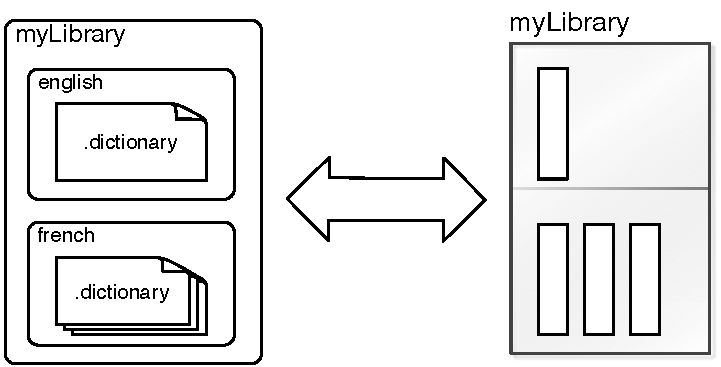
\includegraphics[width=0.7\textwidth]{treeToDictionaryTransformation}
  \caption{Transforming a \texttt{myLibrary} tree into an instance model}
  \label{fig:treeToDictionary}
\end{center}
\end{figure}

\vspace{0.5cm}

Review Part IV, Section 2: \emph{Triple Graph Grammars in a nutshell}, for a detailed and worthwhile overview on how and why TGGs are so useful. In summary,
TGGs form \emph{graph triples} consisting of a source, correspondence, and target component. They are a declarative, rule-based techinique for specifying
the evolution of these three graphs, where the correspondence component can specify and guarantee consistency between elements in the target and source
componenets.

\vspace{0.5cm}

A key idea to keep in mind while creating these rules is the flexibility that this transformation will require. In future \texttt{tree} instances, we may not
know how many subfolders \texttt{myLibrary} will contain, whether or not each \texttt{.dictionary} file will have an author node (as seen in
\texttt{unknown.dictionary}), or how many entries each \texttt{dictionary} will contain. We'll need to avoid situation-specific patterns.

\jumpDual{treeToModel vis}{treeToModel tex}
